\documentclass[english]{article}

% packages
\usepackage[T1]{fontenc}
\usepackage[utf8]{inputenc}
\usepackage{graphicx}
\usepackage{hyperref}
\usepackage{amssymb}
\usepackage{amsmath}
\usepackage[toc,page]{appendix}
\usepackage{listings}

% commands
\newcommand{\sbigotimes}{%
	\mathop{\mathchoice{\textstyle\bigotimes}{\bigotimes}{\bigotimes}{\bigotimes}}%
}
\newcommand{\zeroket}{\begin{pmatrix} 1 \\ 0 \end{pmatrix}}
\newcommand{\oneket}{\begin{pmatrix} 0 \\ 1 \end{pmatrix}}

\graphicspath{{img/}}

\begin{document}
	\title{An Introduction to Quantum Computing for Computer Scientists, with SAT}
	\author{Francesco Piro}
	\maketitle
	
	\begin{abstract}
		This is the paper I have produced during my study of quantum computing for solving the SAT problem...
	\end{abstract}

	% definire meglio la struttura ci sono:
	% definizioni
	% esempi
	% riferimenti al codice nell appendice
	% important conclusions
	
	\section*{Introduction}
	\label{sec:introduction}
	Quantum computation is a wide area involving several disciplines that is having always more success in nowadays applications thanks in particular to the development of the technology and its incredible results. Quantum physics' principles are the fundamentals on which the entire theory is based: thanks to their properties, new architectures allow to define devices that can solve classical problems in surprisingly reduced time and space complexities. However we always have a trade-off to consider, in particular now that these technology are still emerging.\\
	
	This paper aims at giving a description for computer scientists of what a quantum computer is and which are its real impacts and advantages with respect to the classical ones. Hence I will try to provide a description of the state of the art of quantum computing with an approach that allows to understand how from the basic principles of quantum mechanics we are able to have an algorithm that is faster with respect to its classic counterpart. In order to do so in the first chapter (\ref{sec:quantumComputing}) I will start with the basic linear algebra needed to study the quantum physics' principles we need to define a quantum computer. The definition of the \emph{quantum computer} is fundamental both to understand how and algorithm is executed but also to have a comparison with the classic Turing machine that allows us to determine conclusions on computational complexity (chapter \ref{sec:computationalTheory}). In the first chapter we will also have practical examples realized with the \textbf{qiskit library} in order to clarify also with some lines of code the concepts. Once the background on quantum computation and computational theory are well consolidated by the reader, the last chapters provide a practical example that is used to prove the speedup for the particular \textbf{satisfiability problem.} I have used an efficient classical solver for the \emph{k-SAT} as I could compare it with my quantum implementation, both realized in python. In the end I provide some important conclusions for quantum computing that I was able to conclude thanks to my study, in particular in the papers listed in the references.
	
	\section{Quantum Computing}
	\label{sec:quantumComputing}
		This chapter aims at providing first the fundamentals needed in order to deal with quantum mechanics and second at defining a quantum computer thanks to the principles previously identified. With the quantum device we will be able to make a comparison with the classical one to understand with examples how the basic operations are realized in order to use them to implement complete algorithms. Further in the chapter, a section is completely dedicated to the main quantum search algorithm that is fundamental to solve the SAT with a quantum algorithm. Also here we will start from a classical version to compare it with its quantum counterpart. All the arguments related in this chapter, together with the ones in the next (\ref{sec:computationalTheory}) are fundamental to give a significant interpretation to the comparison between the classic and quantum implementation of the algorithm able to solve the \textbf{satisfiability problem} (\ref{sec:sat}).
		
		\subsection{Fundamentals}
		\label{sec:fundamentals}
			The study of quantum computers requires the knowledge of the decimal and binary representation of integers, probability notions and in particular linear algebra fundamental definitions like the ones of: \emph{vectors, spaces, bases, linear systems, tensor product...}. In this section are presented the basic concepts needed to face the quantum physics principles that we need in order to realize our quantum computer. 
			
			\subsubsection{Linear Algebra}
			\label{sec:linearAlgebra}
			Basic principles of linear algebra are assumed to be well known by the reader, I want now to remark only the most important operators and definitions that we need to face the definition of the following quantum mechanical theorems we need to define a quantum device. The most important notions we need to acquire from this section are: \emph{tensor product, Hilbert space, bra-ket notation}.\\
			
			In order to realize a quantum computer we need understand how to define a state that is able to contain information that can be used to obtain a certain objective. As we will see in the next section, the state of a quantum device is a quantum state, thus a mathematical model that lives into a specific \emph{vector state} whose dimension depends on the amount of information it needs to take care of. Typically, significant states contain information that results from the composition of several spaces combined together thanks to a particular operator called tensor product.
			
			\paragraph{Definition (Tensor Product):} \emph{Given two vector spaces V and W over a field K with bases $e_1,..., e_m$ and
$f_1,..., f_n$ respectively, the tensor product $V \otimes W$ is another vector space over K of dimension
mn. The tensor product space is equipped with a bilinear operation $\otimes : V \times W \rightarrow V \otimes W$. The
vector space $V \otimes W$ has basis $e_i \otimes f_j \forall i = 1,...,m, j = 1,...,n$}. \\
			
			Typically we are going to work with complex Euclidean vector spaces of the form $\mathbb{C}^n$ and, by choosing the standard basis in the origin vector spaces, then the tensor product is nothing more than the Kronecker product.
			
			\paragraph{Definition (Kronecker Product):} \emph{Given $A \in \mathbb{C}^{m\times n}$, $B \in \mathbb{C}^{p\times q}$, the Kronecker product $A \otimes B$ is the matrix $D \in \mathbb{C}^{mp\times nq}$ defined as:}
			\begin{center}
				$
				D = A\otimes B =
				\begin{pmatrix}
				a_{11}B & \cdots & a_{1n}B \\
				a_{21}B & \cdots  & a_{2n}B \\
				\vdots & \vdots & \vdots \\
				a_{m1}B & \cdots & a_{mn}B
				\end{pmatrix}
				$
			\end{center}
		
			Now that we know the notions of vector state and Tensor product, we can use them to define an important space (in particular for the SAT problem we are going to study later) called the \textbf{Hilbert space} and denoted with $\mathcal{H}$.
			
			\paragraph{Definition (Hilbert Space):} \emph{Given the complex space $\mathbb{C}$ we define the Hilbert space $\mathcal{H}$ as the (n + 1)-tuple tensor product:}
			\begin{center}
				$
				\mathcal{H} := \sbigotimes_1^{n+1} \mathbb{C}^{2}
				$
			\end{center}
		
			As we said, in the Hilbert space we will carry the discussion of the SAT problem but to understand what the result of this tensor product actually defines we still need to give probably the most important definition. In order to represent a quantum state we use the so called \emph{bra-ket notation} introduced in 1939 by Paul Dirac.
			
			\paragraph{Definition (Dirac/bra-ket Notation):} \emph{Given a complex Euclidean space $\mathbb{S} \equiv \mathbb{C}^{n}$, $|\psi\rangle \in \mathbb{S}$ denotes a column vector, and $\langle\psi| \in \mathbb{S}^{*}$ denotes a row vector that is the conjugate transpose of $|\psi\rangle$, i.i. $\langle\psi| = |\psi\rangle$. The vector $|\psi\rangle$ is also called a ket, while the vector $\langle\psi|$ is also called a bra.} \\
			
			The bra-ket notation allows us to define a quantum state, hence a vector that lives into a particular vector space. Its definition intrinsically defines also the result of combining two states living in the same state with the \textbf{inner product}, straightforwardly obtained from what we have just said: $\langle\psi|\phi\rangle$. This result is fundamental to define spaces that are higher than one only dimension as the Hilbert state presented before. To understand what $\mathcal{H}$ is we can now use two examples where we define the basis of the first two results obtained by doing the tensor product of the complex space $\mathbb{C}^{2}$ with itself. Remember that the basis of a space is the smallest set of linearly independent vectors that can be used to represents all the vectors that belong to that space.
			
			\paragraph{Example 1:} 
			\label{ex:c2}
			\emph{Considering the basic case of $\mathbb{C}^{2}$ the basis can be trivially identified as:}
			\begin{center}
				$|0\rangle = \zeroket \hspace{1cm} |1\rangle = \begin{pmatrix} 0 \\ 1 \end{pmatrix}$
			\end{center}
		
			\paragraph{Example 2:} 
			\label{ex:c4}
			\emph{Considering a single product, thus $\sbigotimes_1^{1} \mathbb{C}^{2} = \mathbb{C}^{2} \otimes \mathbb{C}^{2}$, we obtain the basis by multiplying in all possible ways the vectors of the basis of the previous example. We now have kets of dimension 2, thus vectors with 4 lines and 1 column:}
			\begin{center}
					$
					|00\rangle = |0\rangle \otimes |0\rangle = \zeroket \otimes \zeroket = 
					\begin{pmatrix}
					1\zeroket \vspace{3pt} \\
					0\zeroket
					\end{pmatrix} =
					\begin{pmatrix}
					1 \\ 0 \\ 0 \\ 0
					\end{pmatrix}
					$\vfill
					$
					|01\rangle = |0\rangle \otimes |1\rangle = \zeroket \otimes \oneket = 
					\begin{pmatrix}
					1\oneket \vspace{3pt} \\
					0\oneket
					\end{pmatrix} =
					\begin{pmatrix}
					0 \\ 1 \\ 0 \\ 0
					\end{pmatrix}
					$ \vfill
					$
					|10\rangle = |1\rangle \otimes |0\rangle = \oneket \otimes \zeroket = 
					\begin{pmatrix}
					0\zeroket \vspace{3pt} \\
					1\zeroket
					\end{pmatrix} =
					\begin{pmatrix}
					0 \\ 0 \\ 1 \\ 0
					\end{pmatrix}
					$ \vfill
					$
					|11\rangle = |1\rangle \otimes |1\rangle = \oneket \otimes \oneket = 
					\begin{pmatrix}
					0\oneket \vspace{3pt} \\
					1\oneket
					\end{pmatrix} =
					\begin{pmatrix}
					0 \\ 0 \\ 0 \\ 1
					\end{pmatrix}
					$
			\end{center}
		
			Thanks to these two examples we can generalize to the n + 1 case and obtain the definition of the Hilbert space we gave before. \\
			
			We have now recovered all the fundamentals of linear algebra that are needed in order to start talking of quantum physics, in particular we will begin with the smallest unit of information, the so called \textbf{qubit}.
						
			\subsubsection{Quantum Mechanics}
			\label{sec:quantumMechanics}
				Quantum mechanics is a fundamental theory in physics describing the properties of nature. We do not need entirely its entire power for our purpose but, starting from some basic concepts we will exploit some conclusions that are useful to design an algorithm that is faster than its classical counterpart. As we do when we start studying computer science, we want to identify the smallest, most basic element that allows us to represent the information. From a classical point of view we have the \textbf{bit} whose values can be either 1 or 0. From a quantum point of view, instead, we have the \textbf{qubit}, complex variables that can assume values ranging from 0 to 1 (in modulus), identified in a complex space over a surface called the \emph{Block Sphere}.
				
				\paragraph{Definition (Qubit:)} \emph{The qubit is the smallest unit of measurement used to quantify information in quantum computing. It identifies the bit in a superposition, hence both 0 and 1 values are considered. Formally it is a vector of the space $\mathbb{C}^{2}$ represented as a linear combination of the elements contained in its basis (\ref{ex:c2}). A qubit $\psi$, with $\alpha_0,\alpha_1\in\mathbb{C}$, is defined as:}\\
				\begin{center}
					$
					|\psi\rangle = \alpha_0 |0\rangle + \alpha_1 |1\rangle = \alpha_0\zeroket + \alpha_1\oneket
					$
				\end{center}
				
				To understand better the definition of the qubit we now provide its representation in a tridimensional space whose directions are obtained from basic linear algebra principles that are not now relevant. We now just need to understand that, thanks to the coefficients $\alpha_0$ and $\alpha_1$ belonging to the complex space $\mathbb{C}$ we are able to consider the basic element of our computation as one of the infinite points that live over the surface of a sphere. We can grasp in this concept a first hint in the advantages that quantum states provide with respect their classic counterpart.
				
				\paragraph{Definition (Block Sphere):} \emph{The Block Sphere is the geometrical representation of the pure state space of a two-level quantum mechanical system. In other words it represents all the possible vectors that can be obtained by combining the vectors of the basis for a quantum register of 1 qubit.}\\
				
				Consider the following examples to understand how vectors are represented in the Bloch sphere; we present the trivial cases for both $|0\rangle$ and $|1\rangle$ and the respective orthogonal vectors identifying the x and y axes.
				
				\newpage
				
				\paragraph{Example 3:} \emph{Consider the qubit $\psi$, with $\alpha_0,\alpha_1\in\mathbb{C}$, such that: 	$|\psi\rangle = \alpha_0 |0\rangle + \alpha_1 |1\rangle$. (Check code at \ref{c:example3})}
				
				\begin{enumerate}
					\centering
					\begin{figure}[h]
						\begin{minipage}{0.4\textwidth}
							\item $\alpha_0=1, \;\alpha_1=0$
							\centering
							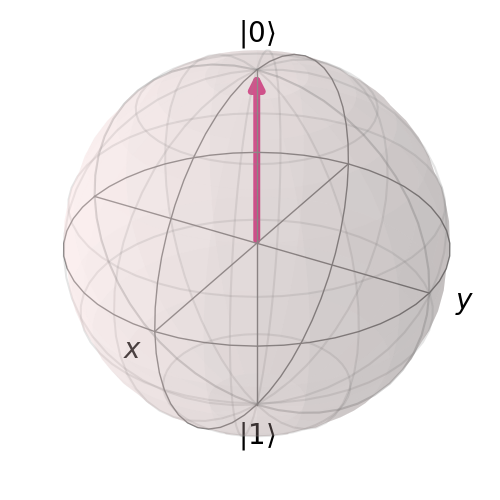
\includegraphics[scale=0.4]{zeroket.png}
							\caption{$|\psi\rangle= |0\rangle$}
						\end{minipage} \hfill
						\begin{minipage}{0.4\textwidth}
							\item $\alpha_0=0, \;\alpha_1=1$
							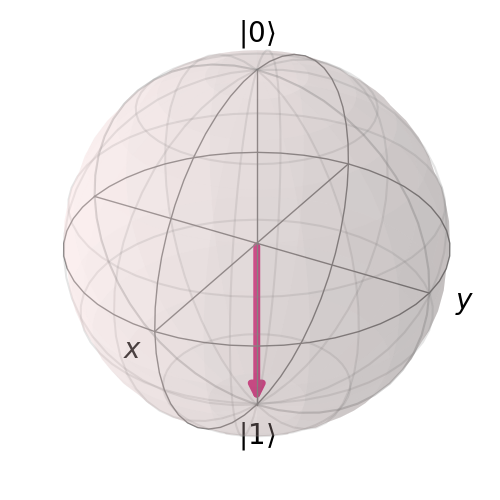
\includegraphics[scale=0.4]{oneket.png}
							\caption{$|\psi\rangle= |1\rangle$}
						\end{minipage}
					\end{figure}
					\begin{figure}[h]
						\begin{minipage}{0.4\textwidth}
							\item $\alpha_0=\frac{1}{\sqrt{2}}, \;\alpha_1=\frac{1}{\sqrt{2}}$
							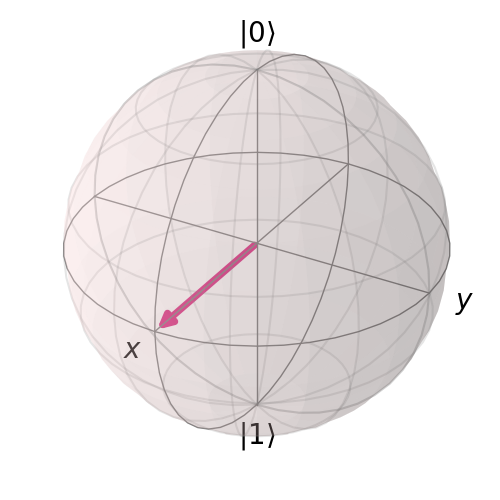
\includegraphics[scale=0.4]{xket.png}
							\caption{$|\psi\rangle = \frac{1}{\sqrt{2}}(|0\rangle+|1\rangle)$}
						\end{minipage} \hfill
						\begin{minipage}{0.4\textwidth}
							\item $\alpha_0=\frac{1}{\sqrt{2}}, \;\alpha_1=\frac{i}{\sqrt{2}}$
							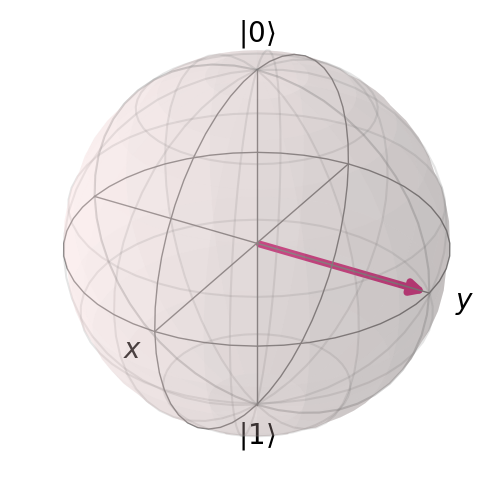
\includegraphics[scale=0.4]{yket.png}
							\caption{$|\psi\rangle = \frac{1}{\sqrt{2}}(|0\rangle+i|1\rangle)$}
						\end{minipage}
					\end{figure}
				\end{enumerate}
			
			Obviously we can also represent vectors that belong to spaces with a higher dimension than 2, in this case we will have their representation over a hypersphere (check the plot\_bloch\_multivector method in the qiskit library). As in classical computer we haver registers, defined as a sequence of bits, in quantum computing we have \emph{quantum-registers} composed of a sequence of qubits. Typically a quantum computer has a single quantum-register made up of qubits (see section \ref{sec:quantumComputer}). It is now important to remark the first important conclusion on quantum computing, that derives from the definition of quantum-register that we have just provided. We see that $\sbigotimes_1^{n+1} \mathbb{C}^{2}$ is a $2^{n}$ dimensional space. This is sharp in contrast with what happens for classical registers: given n classical bits, their state is a binary string in $\{0,1\}^{n}$, thus an n-dimensional space. In other words:
			
			\paragraph{Conclusion 1:} \emph{the dimension of the state space of quantum registers grows exponentially in the number of qubits, whereas the dimension of the state space of classical registers grows linearly in the number of bits.}
			
			\subsubsection{Superposition}
			\label{sec:superposition}
			
			\subsubsection{Entanglement}
			\label{sec:entanglement}
			
			\subsubsection{The Quantum Computer}
			\label{sec:quantumComputer}
			
		\subsection{Grover's Algorithm}
		\label{sec:grover}
		
	\section{Computational Theory}
	\label{sec:computationalTheory}
		\subsection{SAT Problem}
		\label{sec:sat}
		
	\section{SAT Implementation}
	\label{sec:satImpl}
		\subsection{Classical}
		\label{sec:satClassical}
		
		\subsection{Quantum}
		\label{sec:satQuantum}
		
		\subsection{Classical vs. Quantum}
		\label{sec:satCsatQ}
		
	\section{Conclusions}
	\label{sec:conclusions}
	
	\begin{appendices}
		\section{Qiskit}
		\label{sec:qiskit}
		
		\section{Code with Qiskit}
		This section contains the list of the snippets of code needed to represent the examples used in the paper. To replicate them consider ti import the following libraries:
		\lstinputlisting[language=python]{code/imports.py}
		
		\label{sec:codeWithQiskit}
			\begin{enumerate}
				\item \label{c:example3} \lstinputlisting[language=python]{code/example3.py}
			\end{enumerate}
	\end{appendices}
	
	\clearpage
	\bibliographystyle{plain}
	\nocite{*}
	\bibliography{main.bib}
\end{document}

